\documentclass[conference]{IEEEtran}

\usepackage{graphicx}
\usepackage{listings}
\usepackage{xcolor}

\lstdefinelanguage{json}{
    basicstyle=\ttfamily\small,
    numbers=none,
    showstringspaces=false,
    breaklines=true,
    frame=single,
    morestring=[b]",
    morecomment=[l]{//},
    stringstyle=\color{black},
    keywordstyle=\color{blue},
    commentstyle=\color{gray},
    literate=
     *{0}{{{\color{blue}0}}}{1}
      {1}{{{\color{blue}1}}}{1}
      {2}{{{\color{blue}2}}}{1}
      {3}{{{\color{blue}3}}}{1}
      {4}{{{\color{blue}4}}}{1}
      {5}{{{\color{blue}5}}}{1}
      {6}{{{\color{blue}6}}}{1}
      {7}{{{\color{blue}7}}}{1}
      {8}{{{\color{blue}8}}}{1}
      {9}{{{\color{blue}9}}}{1}
      {:}{{{\color{black}:}}}{1}
      {,}{{{\color{black},}}}{1}
      {\{}{{{\color{black}\{}}}{1}
      {\}}{{{\color{black}\}}}}{1}
}

\lstdefinelanguage{kotlin}{
    keywords={fun,val,var,if,else,for,while,return,null,true,false,class,object,package,import},
    keywordstyle=\color{blue}\bfseries,
    ndkeywords={},
    ndkeywordstyle=\color{darkgray}\bfseries,
    identifierstyle=\color{black},
    sensitive=true,
    comment=[l]{//},
    morecomment=[s]{/*}{*/},
    commentstyle=\color{gray}\ttfamily,
    stringstyle=\color{red}\ttfamily,
    morestring=[b]",
    morestring=[s]{"""*}{*"""},
    basicstyle=\ttfamily\small,
    breaklines=true,
    showstringspaces=false,
    frame=single
}

\usepackage{url}

\definecolor{codegray}{gray}{0.9}

\lstset{
    backgroundcolor=\color{codegray},
    basicstyle=\ttfamily\small,
    breaklines=true,
    frame=single,
    captionpos=t,
    showspaces=false,
    showtabs=false,
    showstringspaces=false,
    columns=flexible
}

\usepackage{caption}

\captionsetup[lstlisting]{
    position=top,
    skip=6pt
}

\usepackage{float}

\title{Demonstration of Load Balancing in a Distributed System}

\author{
\IEEEauthorblockN{Dimitar Betinski}
\IEEEauthorblockA{
Faculty of Computer Science and Engineering\\
Distributed Systems\\
Index No: 175030\\
Email: dimitar.betinski@students.finki.ukim.mk
}
}

\begin{document}
\maketitle

\begin{abstract}
This paper demonstrates load balancing in a distributed system with multiple replicated backend services and a round-robin load balancer. Backend services run on Google Cloud Platform (GCP) VMs, while the load balancer is on a DigitalOcean instance, illustrating cross-platform request routing. The system showcases request distribution, stateless service design, and fault tolerance.
\end{abstract}

\begin{IEEEkeywords}
Distributed systems, load balancing, round-robin, cloud computing, stateless services
\end{IEEEkeywords}

\section{Introduction}
Distributed systems rely on service replication and load balancing for scalability and reliability. A load balancer distributes client requests across backend servers to prevent bottlenecks. This report presents a simple system where identical backend services respond via a round-robin load balancer.

\section{System Architecture}
The system has three backend VMs on GCP and an external load balancer on DigitalOcean, demonstrating cross-cloud request routing. This setup highlights request distribution, stateless design, and fault tolerance.

\begin{figure}[H]
\centering
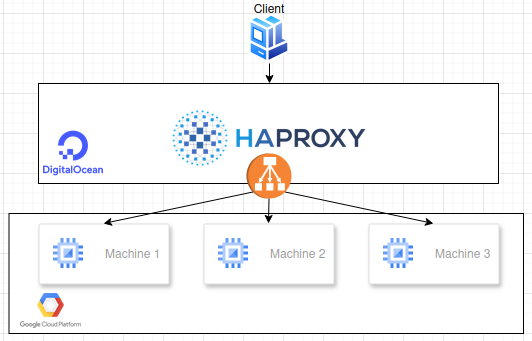
\includegraphics[width=0.45\textwidth]{architectureDO.png}
\caption{System architecture with external load balancer and replicated backend services}
\label{fig:architecture}
\end{figure}

\section{Backend Service Implementation}

Each backend node runs the same Kotlin-based REST API implemented using the Ktor framework. The service is intentionally stateless and exposes two HTTP endpoints: an information endpoint used to demonstrate request distribution and a health-check endpoint used by the load balancer to determine backend availability.

\begin{lstlisting}[language=Kotlin, caption=Ktor routing implementation for backend service]
package com.dimitry4now

import com.dimitry4now.model.InfoResponse
import com.dimitry4now.model.Student
import io.ktor.server.application.*
import io.ktor.server.response.*
import io.ktor.server.routing.*
import kotlinx.coroutines.delay
import java.time.LocalDate

fun Application.configureRouting() {
  val machineName = System.getenv("MACHINE_NAME") ?: "machineX"
  val machineEnabled = System.getenv("MACHINE_ENABLED")?.toBoolean() ?: true
  val student = Student("Dimitar", "Betinski", "175030")
  val targetPrimes = System.getenv("TARGET_PRIMES")?.toInt() ?: 200

  routing {
    fun isPrime(n: Long): Boolean {
      if (n < 2) return false
      if (n % 2L == 0L) return n == 2L
      var i = 3L
      while (i * i <= n) {
        if (n % i == 0L) return false
        i += 2
      }
      return true
    }

    get("/work-cpu-bound") {
      val rnd = java.util.Random()
      var primesFound = 0
      val targetPrimes = targetPrimes

      while (primesFound < targetPrimes) {
        val candidate = rnd.nextLong(10_000_000L, 50_000_000L)
        if (isPrime(candidate)) {
          primesFound++
        }
      }

      call.respond(
        InfoResponse(
          student = student,
          date = LocalDate.now().toString(),
          machine = machineName
        )
      )
    }

    get("/health") {
      if (machineEnabled) {
        call.respondText("OK")
      } else {
        call.respondText("DOWN", status = io.ktor.http.HttpStatusCode.ServiceUnavailable)
      }
    }
  }
}
\end{lstlisting}

The \texttt{/work-cpu-bound} endpoint returns a JSON response containing static student information, the current date, and the identifier of the responding machine. The machine identifier is injected through an environment variable, allowing the same application binary to be deployed across all backend instances. There is also a calculation for prime numbers to simulate random delay(3s-5s).

The \texttt{/health} endpoint provides a lightweight health-check mechanism. By modifying an environment variable, backend instances can be logically disabled without stopping the service, enabling controlled fault simulation during testing.

\section{Backend Deployment and Execution}

The backend service was deployed on multiple Ubuntu Server virtual machines hosted on Google Cloud Platform. The application was initially built using the standard Gradle build process:

\begin{lstlisting}[language=bash, caption=Initial Gradle build command]
./gradlew clean build
\end{lstlisting}

This build produced a standard JAR artifact, which was transferred to a backend virtual machine and executed using the Java runtime. However, the application failed to start because the generated artifact did not include a defined entry point in its manifest file and therefore could not be executed as a standalone application.

To resolve this issue, the build configuration was modified to generate a fat (uber) JAR containing all required dependencies and a properly defined main entry point for the Ktor server. After rebuilding the application, the resulting artifact could be executed directly using the Java runtime.

Each virtual machine was configured with the required Java runtime environment and a dedicated non-privileged system user. The backend service was deployed under the \texttt{/opt/ktor} directory and managed using systemd to ensure reliable startup, automatic restarts, and integration with the operating system’s service management.

\subsection{systemd Service Configuration}

The backend application was executed as a system-managed service using systemd. Listing~\ref{lst:systemd} shows the unit file used to manage the backend service.

\begin{lstlisting}[language=bash, caption=systemd service definition for the Ktor backend, label=lst:systemd]
[Unit]
Description=Ktor Backend Service
After=network.target

[Service]
Type=simple
User=ktor
WorkingDirectory=/opt/ktor

ExecStart=/usr/bin/java \
  -Xms256m \
  -Xmx512m \
  -jar /opt/ktor/app.jar

Restart=always
RestartSec=5

Environment=MACHINE_NAME=Machine1
Environment=MACHINE_ENABLED=true
Environment=TARGET_PRIMES=14500

[Install]
WantedBy=multi-user.target
\end{lstlisting}

The service could not be started using the default build, due to the way Kotlin compiles and packages applications on the JVM. To resolve this issue, it was necessary to build a fat JAR that includes all dependencies. The service was successfully started after executing the following build command:

\begin{lstlisting}[language=bash, caption=The actual build command that worked, label=lst:fatjar]
./gradlew clean buildFatJar
\end{lstlisting}

The \texttt{MACHINE\_NAME} environment variable is configured uniquely on each backend instance, allowing the same application binary to be deployed across all machines while still identifying the responding node. After deployment, the service was verified locally on each virtual machine using direct HTTP requests before being integrated with the load balancer.

\begin{lstlisting}[language=bash, caption=Local backend verification using curl]
curl http://localhost:8080/work-cpu-bound | jq
\end{lstlisting}

The output of the command for \texttt{Machine1} is shown in Listing~\ref{lst:curl-output}:

\begin{lstlisting}[language=json, caption=Sample JSON response from the backend, label=lst:curl-output]
{
  "student": {
    "name": "Dimitar",
    "surname": "Betinski",
    "index": "175030"
  },
  "date": "2026-01-15",
  "machine": "Machine1"
}
\end{lstlisting}

The same deployment procedure was repeated for all remaining backend machines, resulting in multiple identical service instances ready to operate behind the load balancer.

\section{Load Balancer Configuration}

The load balancer was implemented using HAProxy on a DigitalOcean droplet. HAProxy was installed and enabled as a system service to automatically start on boot. This ensures that backend request distribution continues even after a server restart. The installation commands used were:

\begin{lstlisting}[language=bash, caption=Installing and enabling HAProxy on Ubuntu]
sudo apt update
sudo apt install haproxy -y
sudo systemctl enable haproxy
sudo systemctl start haproxy
sudo systemctl status haproxy
\end{lstlisting}

The HAProxy configuration was set up to distribute incoming HTTP requests to the backend servers using the round-robin algorithm. A frontend listener was bound to port 80, and a backend section was configured to perform **health checks** by querying the \texttt{/health} endpoint of each backend. Only servers returning a successful status code (200 OK) are considered healthy and receive requests. The configuration is shown in Listing~\ref{lst:haproxy}.

\begin{lstlisting}[language=bash, caption=HAProxy frontend and backend configuration with health checks, label=lst:haproxy]
frontend http_front
    bind *:80
    default_backend backend_servers

backend backend_servers
    balance roundrobin
    option httpchk GET /health
    http-check expect status 200
    server machine1 34.89.77.210:8080 check
    server machine2 35.246.73.120:8080 check
    server machine3 35.246.96.169:8080 check
\end{lstlisting}

This configuration ensures that requests are distributed fairly among the three backend servers, and unhealthy servers are automatically excluded until they recover.

\section{Demonstration and Results}

To demonstrate the correct operation of the load balancer and the backend services, a custom monitoring script was written. This script sequentially queries the load balancer endpoint and records which backend machine responds, allowing us to observe the round-robin behavior in real time. The script is shown below:

\begin{lstlisting}[language=bash, caption=Custom monitoring script for observing backend responses, label=lst:monitor-script]
#!/bin/bash

URL="${1:-http://164.90.240.114/work-cpu-bound}"
INTERVAL="${2:-1}"
i=1

echo "Monitoring $URL every $INTERVAL seconds..."
echo "Request No / Machine"

while true; do
    MACHINE=$(curl -s "$URL" | jq -r '.machine')
    echo "$i / $MACHINE"
    i=$((i+1))
    sleep "$INTERVAL"
done
\end{lstlisting}

The script can be executed with the load balancer's public IP as an argument, for example:

\begin{lstlisting}[language=bash, caption=Running the monitoring script against the load balancer]
./monitor_proxy.sh http://164.90.240.114/info 1
\end{lstlisting}

Figure~\ref{fig:rr-action} shows a screenshot of the script output in action, visually illustrating the alternating responses from the backend nodes.

\begin{figure}[H]
\centering
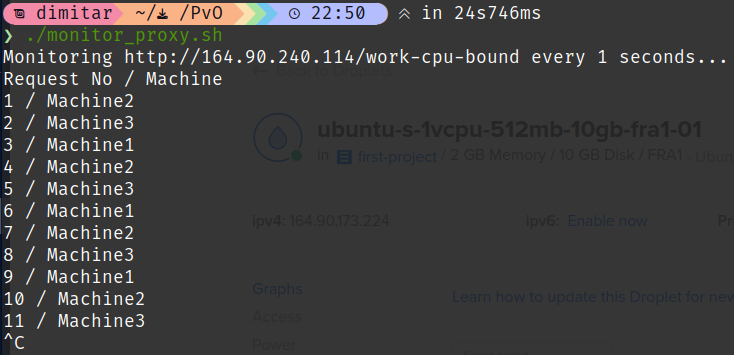
\includegraphics[width=0.45\textwidth]{rr_action.png}
\caption{Monitoring script showing sequential responses from backend servers}
\label{fig:rr-action}
\end{figure}

This demonstrates that the round-robin load balancing algorithm is functioning correctly. The \texttt{Machine} field in the JSON response makes it easy to identify which instance handled each request.

\subsection{Performance Evaluation Using k6}

After validating the correct round-robin behavior of the load balancer, performance testing was carried out using \texttt{k6}, a load testing tool developed by Grafana. The objective of these tests was to measure execution time and throughput under load, and to evaluate the speedup achieved as additional backend machines were enabled.

The k6 tool was used to generate a consistent and repeatable load against the load balancer endpoint. Three configurations were evaluated:
\begin{itemize}
    \item One backend machine (baseline)
    \item Two backend machines active
    \item Three backend machines active
\end{itemize}

The raw performance metrics produced by k6 were collected for each configuration. These results were then post-processed using custom Python scripts to compute aggregate metrics and generate plots for execution time, speedup, and throughput.

Figure~\ref{fig:exec-time} shows the average execution time observed for each configuration. As additional backend machines are introduced, the execution time decreases, indicating improved parallel handling of requests.

\begin{figure}[H]
\centering
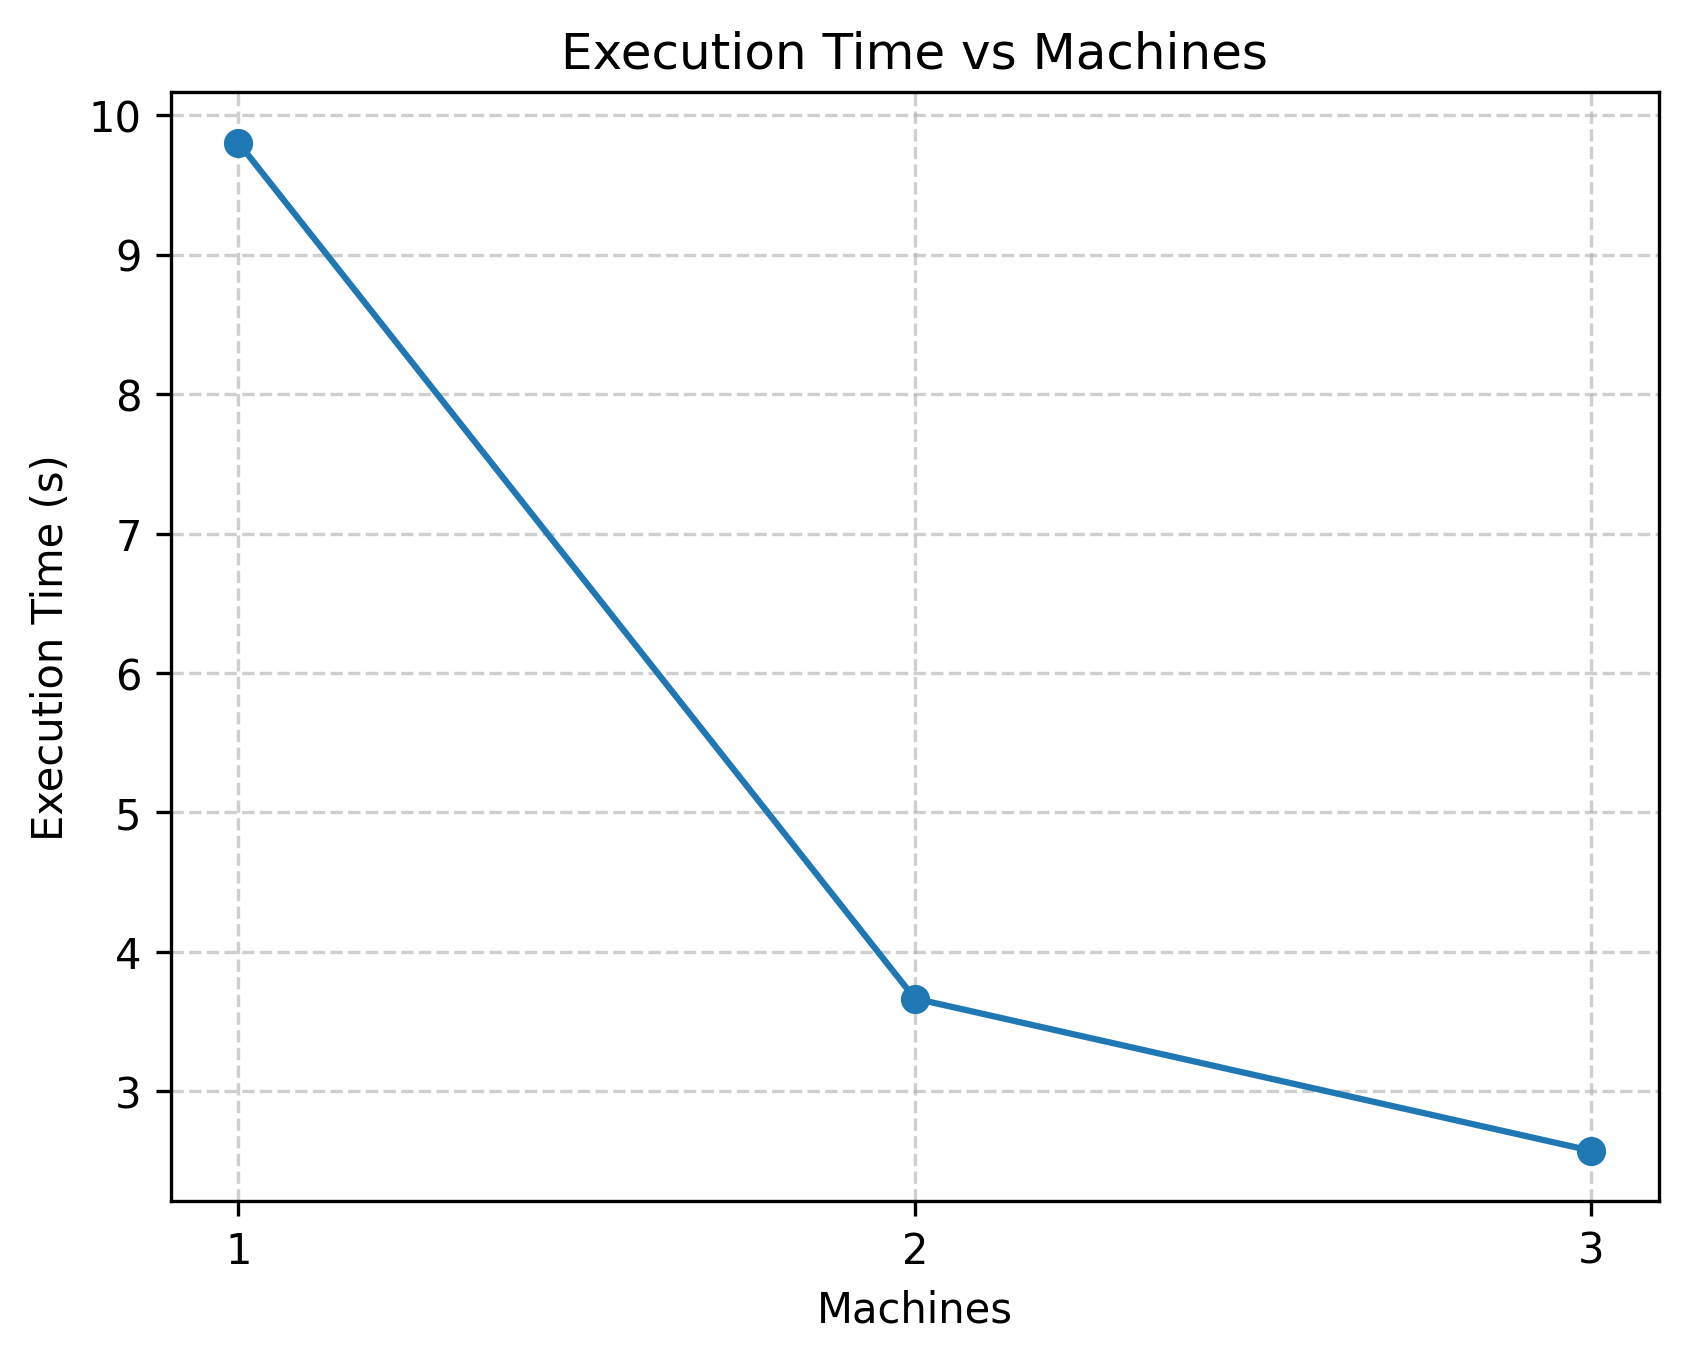
\includegraphics[width=0.48\textwidth]{exec_time.png}
\caption{Average execution time for different numbers of backend machines}
\label{fig:exec-time}
\end{figure}

Figure~\ref{fig:speedup} presents the measured speedup, computed relative to the single-machine baseline. The results demonstrate that adding backend machines leads to near-linear performance gains, confirming the effectiveness of the load balancer under increased concurrency.

\begin{figure}[H]
\centering
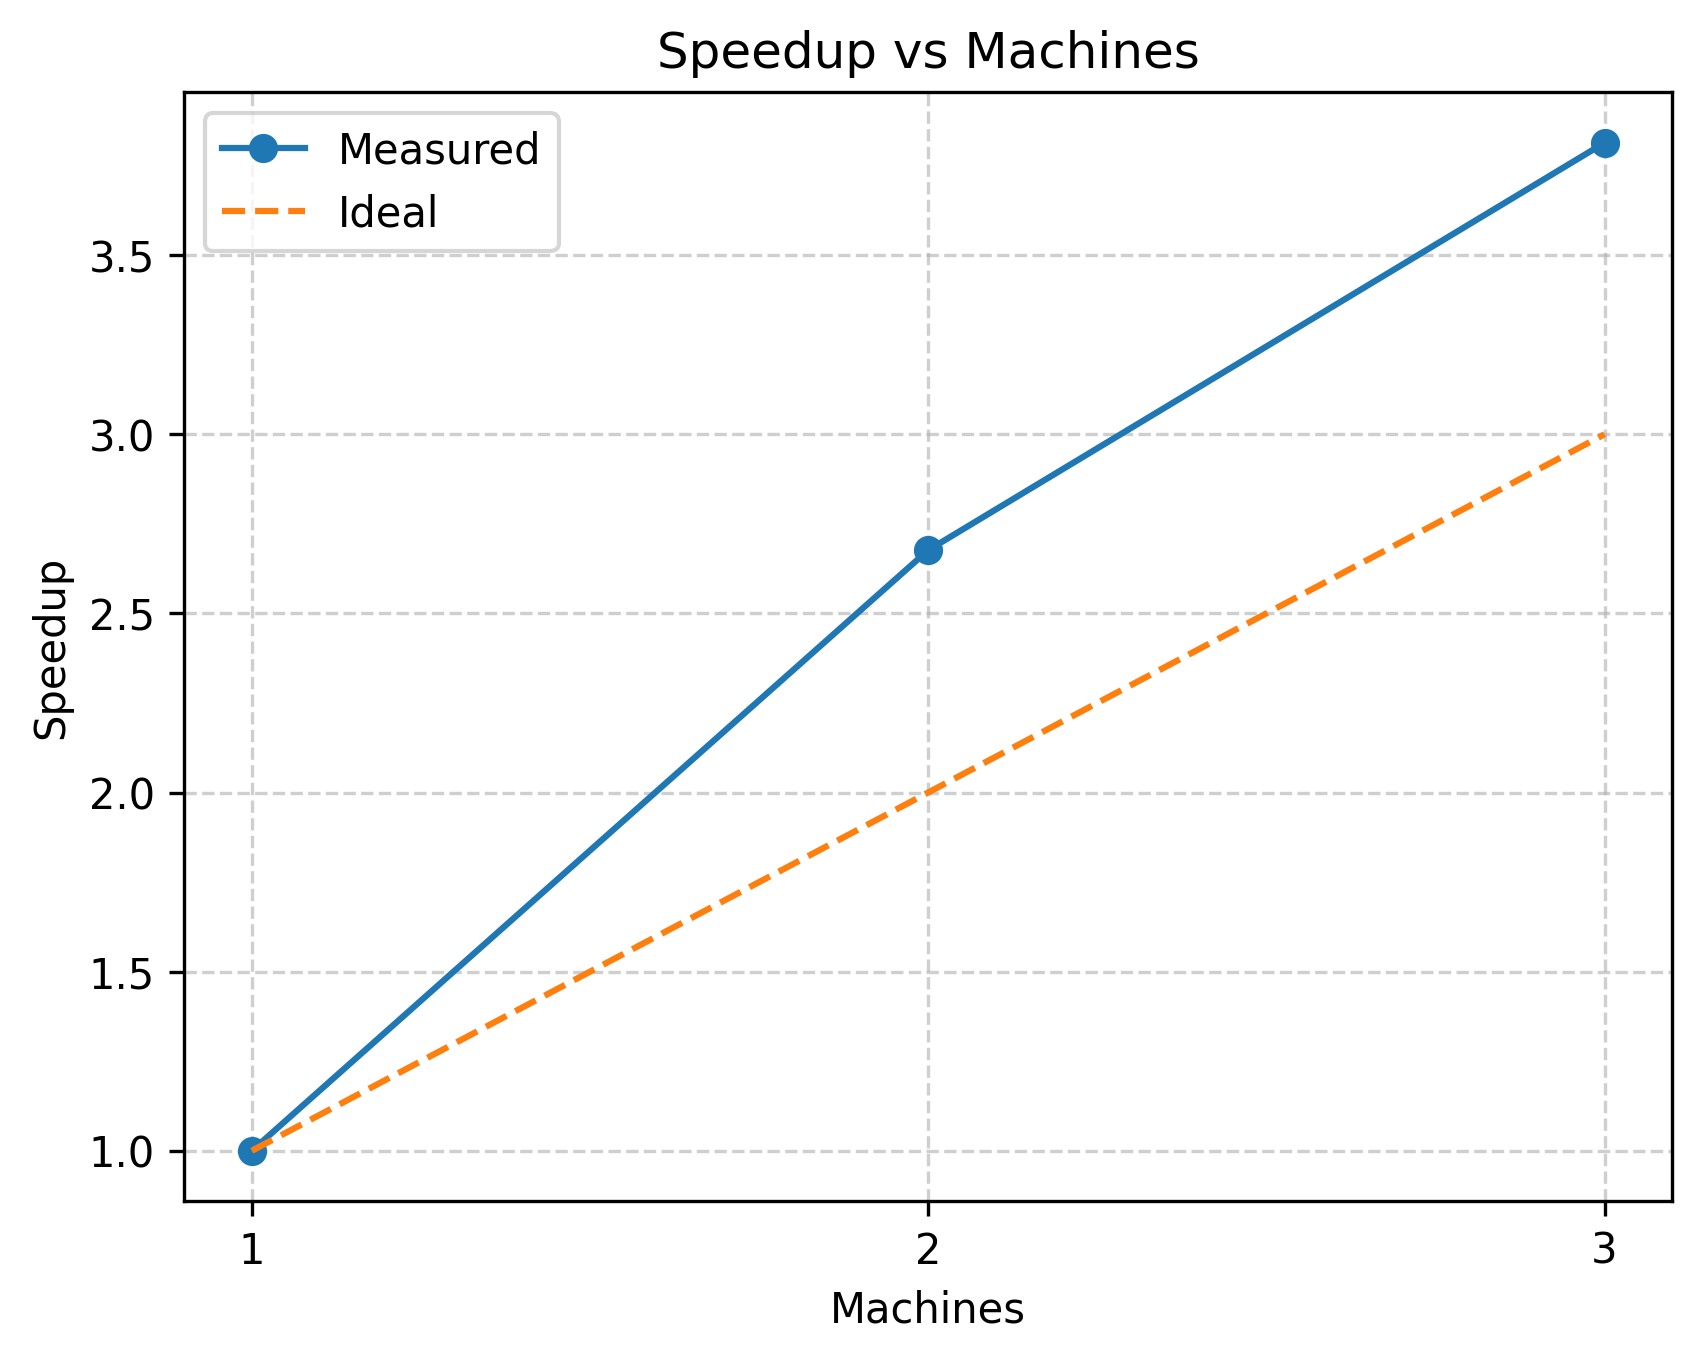
\includegraphics[width=0.48\textwidth]{speedup.png}
\caption{Measured speedup with one, two, and three backend machines}
\label{fig:speedup}
\end{figure}

Figure~\ref{fig:throughput} illustrates the system throughput in terms of processed requests per second. Throughput increases as more backend machines are enabled, showing that the system scales positively with additional resources.

\begin{figure}[H]
\centering
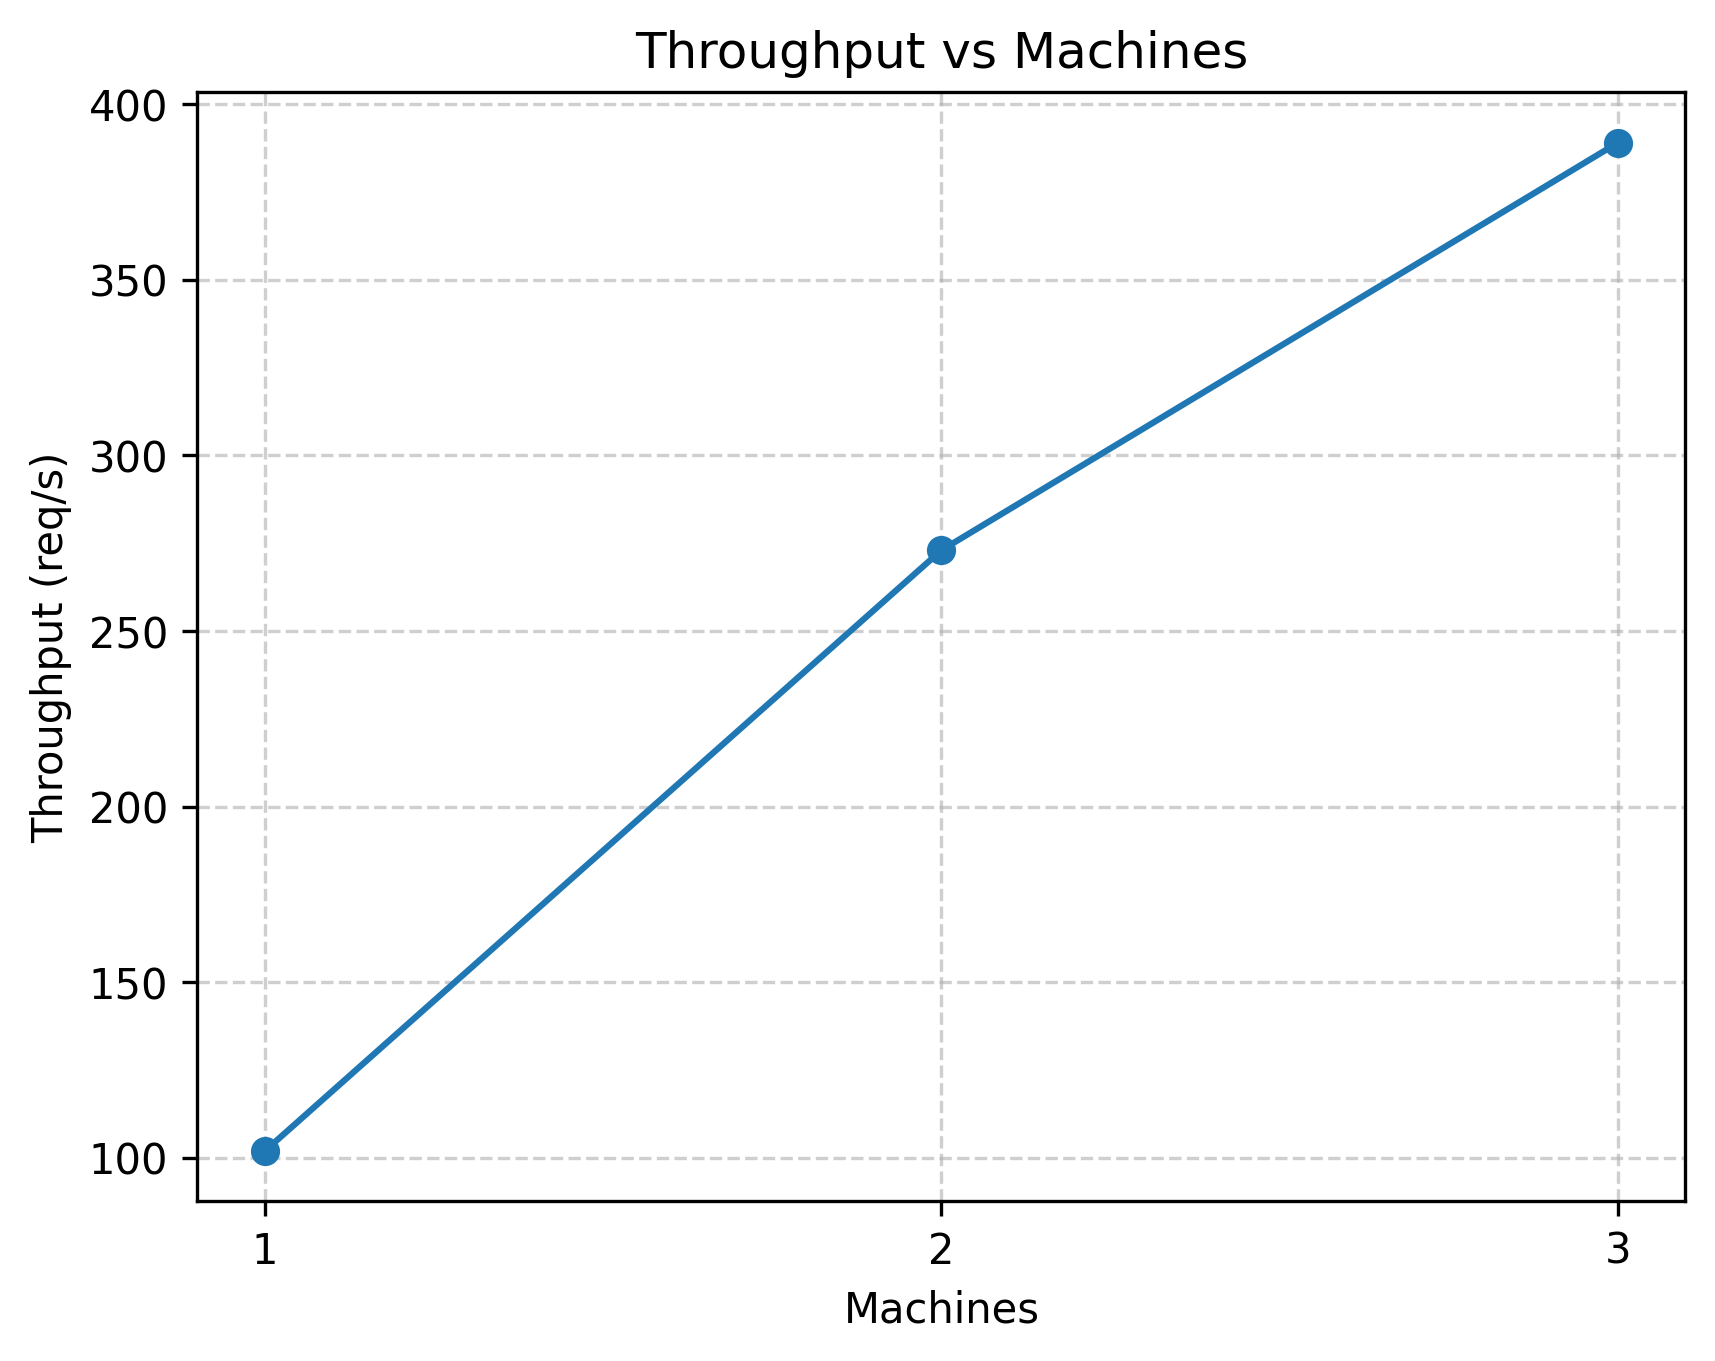
\includegraphics[width=0.48\textwidth]{throughput.png}
\caption{System throughput for different backend configurations}
\label{fig:throughput}
\end{figure}

In addition to the plotted metrics, k6 provides detailed textual execution summaries after each test run. Figures~\ref{fig:k6-result-1}, \ref{fig:k6-result-2}, and \ref{fig:k6-result-3} show the k6 results for the one-, two-, and three-machine configurations, respectively.

\begin{figure}[H]
\centering
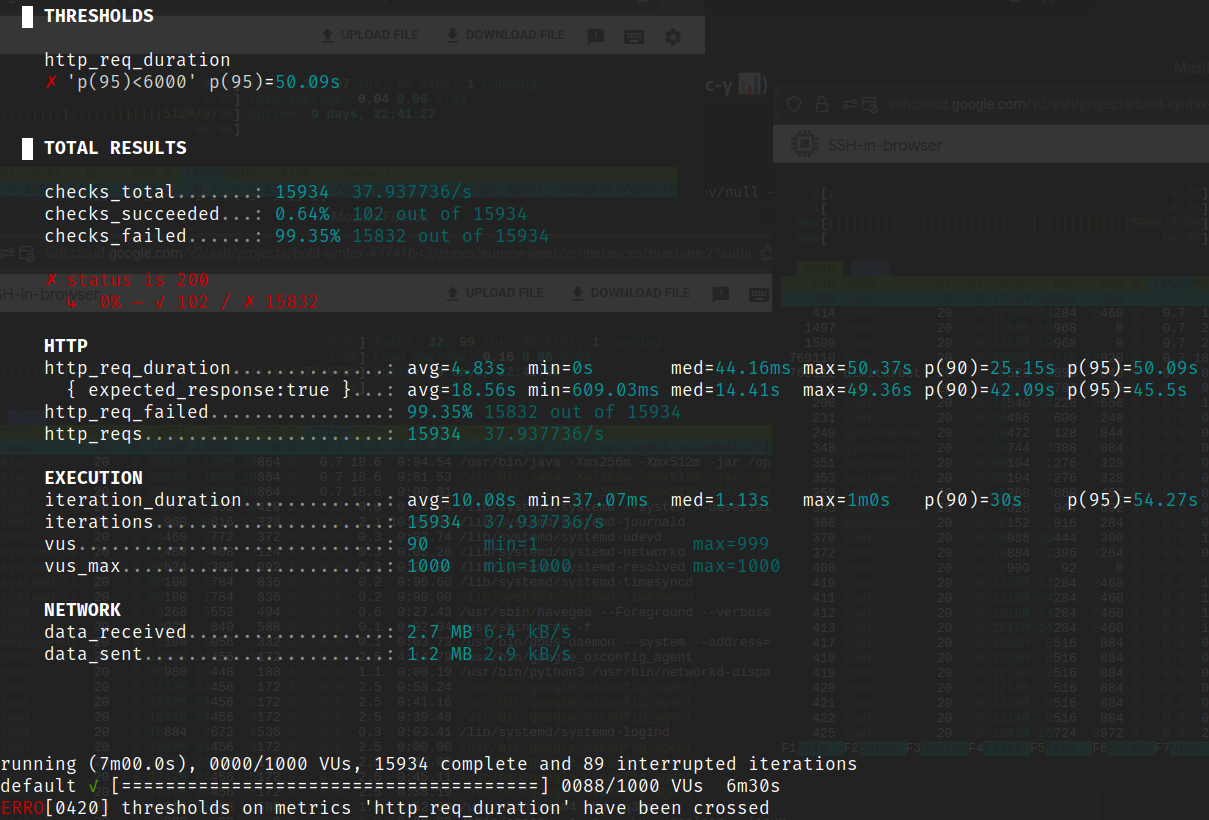
\includegraphics[width=0.48\textwidth]{oneMachineRunningK6.png}
\caption{k6 execution summary with one backend machine (baseline)}
\label{fig:k6-result-1}
\end{figure}

\begin{figure}[H]
\centering
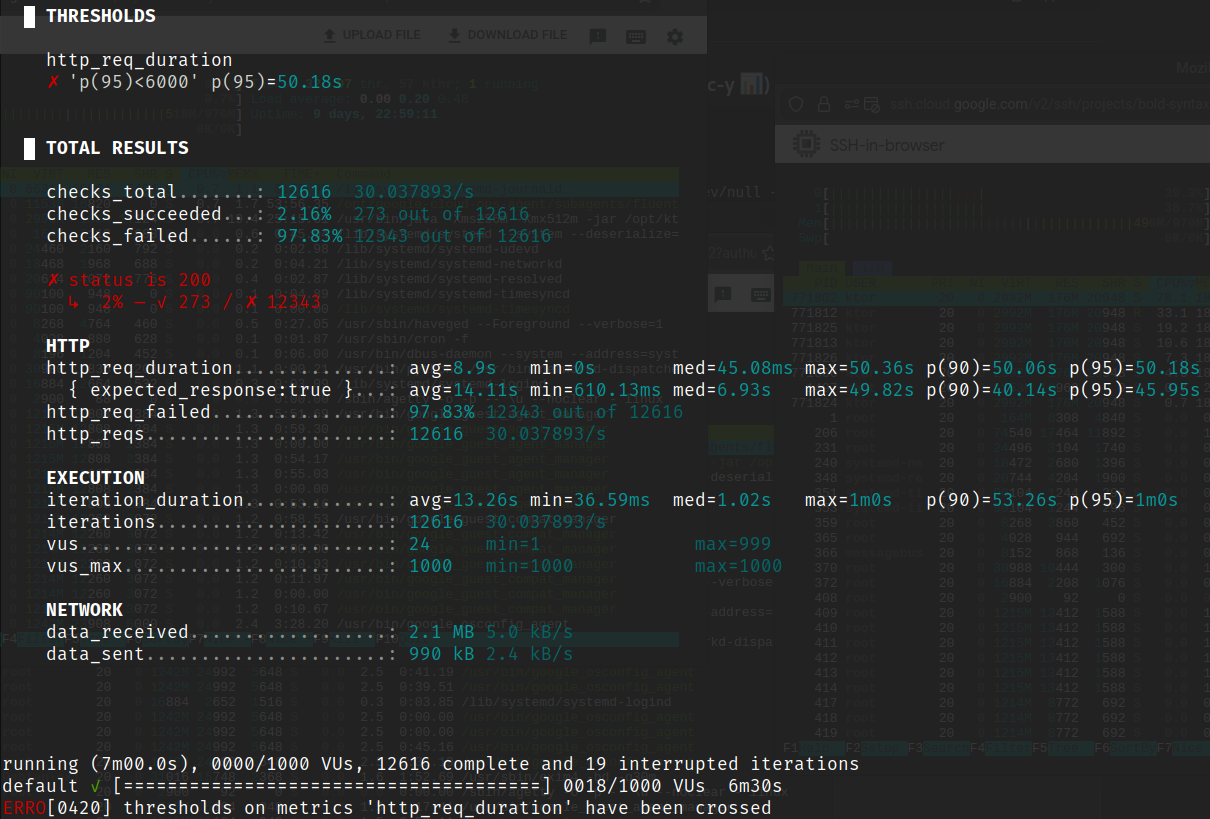
\includegraphics[width=0.48\textwidth]{twoMachinesRunningK6.png}
\caption{k6 execution summary with two backend machines}
\label{fig:k6-result-2}
\end{figure}

\begin{figure}[H]
\centering
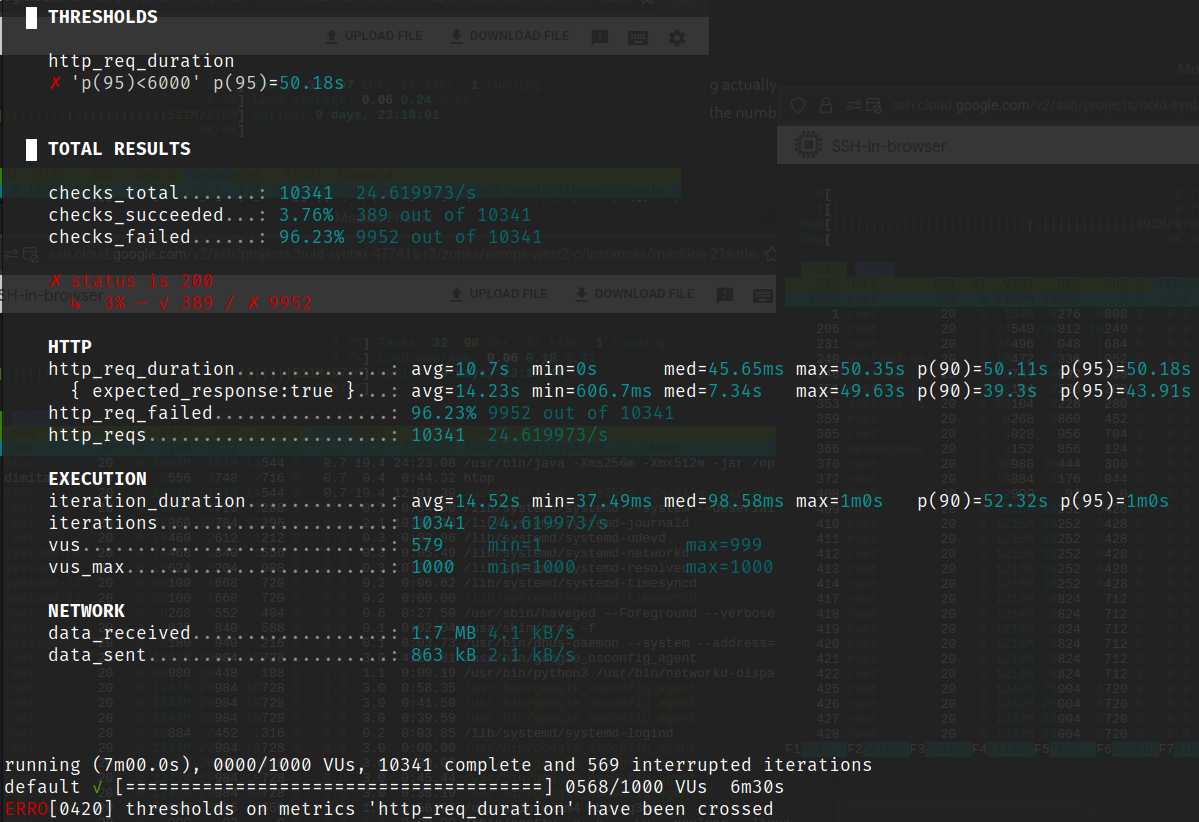
\includegraphics[width=0.48\textwidth]{threeMachinesRunningK6.png}
\caption{k6 execution summary with three backend machines}
\label{fig:k6-result-3}
\end{figure}

Overall, the results confirm that the system benefits from horizontal scaling. The reduction in execution time, increased throughput, and observed speedup collectively demonstrate that the load balancer effectively distributes incoming requests across the available backend machines.

\section{Discussion}

The initial deployment failure highlighted the critical importance of correct artifact packaging in distributed environments, particularly when deploying JVM-based services as system-managed processes rather than running them in development mode. Creating a proper fat JAR and configuring a systemd service ensured reliable execution across all backend nodes.

The implemented system effectively demonstrates several fundamental concepts of distributed systems:

\begin{itemize}
    \item \textbf{Stateless services:} Each backend instance handles requests independently, with no session state stored locally, allowing any node to respond to any request.
    \item \textbf{Horizontal scalability:} Additional backend instances can be deployed seamlessly behind the load balancer to handle increased load.
    \item \textbf{Load distribution and fault tolerance:} The round-robin algorithm ensures fair distribution of requests, and the health checks automatically remove unavailable nodes from the routing pool.
\end{itemize}

\subsection{Scalability}

Scalability was evaluated by increasing the number of concurrent requests using the k6 load testing tool and progressively enabling additional backend machines. The performance results show a clear reduction in average execution time and an increase in overall throughput as the number of backend instances increased from one to three.

The measured speedup demonstrates that the system scales positively under increased load. While the speedup is not perfectly linear, which is expected due to coordination overhead, load balancer processing, and shared infrastructure limits, the results indicate that the system can effectively utilize additional backend resources to handle higher user demand.

\subsection{Elasticity}

Elasticity refers to the system’s ability to adapt to sudden changes in load. In this implementation, elasticity was tested by dynamically enabling and disabling backend machines using environment variables while the system was under load. The HAProxy health-check mechanism detected unavailable instances and automatically excluded them from the request pool.

When disabled instances were re-enabled, they were seamlessly reintegrated into the load balancing rotation without requiring service restarts or manual reconfiguration. This behavior demonstrates that the system can tolerate abrupt fluctuations in available resources and user demand, maintaining service availability and stable performance during transient conditions.

\subsection{Cost Analysis}

From a cost perspective, the system benefits from its use of lightweight virtual machines and stateless service design. Backend services can be scaled horizontally by adding or removing virtual machines, allowing operational costs to be closely aligned with current demand.

Running backend services on separate virtual machines introduces additional infrastructure costs; however, these costs are offset by improved performance, fault tolerance, and availability. Furthermore, the use of open-source tools such as HAProxy, k6, and Kotlin-based frameworks minimizes software licensing expenses.

In a production environment, this architecture enables cost optimization strategies such as scaling down during periods of low demand and scaling up only when necessary. As a result, the system provides a balanced trade-off between performance, resilience, and operational cost.

\section{Conclusion}

This project demonstrates a practical implementation of load balancing in a distributed system using replicated backend services and an external HAProxy load balancer. The round-robin algorithm guarantees equitable request distribution, while the stateless architecture allows for horizontal scaling and fault tolerance.

The experience gained underscores the importance of correct deployment practices, automated health checks, and monitoring tools in maintaining a robust distributed system. Future improvements could include:

\begin{itemize}
    \item Dynamic scaling of backend instances based on load.
    \item Enhanced monitoring dashboards to visualize traffic patterns.
    \item Exploration of more advanced load balancing strategies, such as least-connections or weighted distribution.
\end{itemize}

By integrating these enhancements, the system could better support production-level workloads while maintaining reliability and performance.

\begin{thebibliography}{1}

\bibitem{tanenbaum}
A. S. Tanenbaum and M. van Steen, \emph{Distributed Systems: Principles and Paradigms}, 2nd ed. Pearson, 2007.

\bibitem{haproxy}
HAProxy Documentation. [Online]. Available: \url{https://www.haproxy.org}

\bibitem{gcp}
Google Cloud Platform Documentation. [Online]. Available: \url{https://cloud.google.com}

\end{thebibliography}

\end{document}
